% Rapport du Projet 3 : moteur multimodal de recherche et d'assistance (texte + image + audio)
% Compilation : make report   (pdflatex + bibtex). Les figures viennent de ../artifacts/figures/ (make figures).
\documentclass[11pt,a4paper]{article}
\usepackage[utf8]{inputenc}
\usepackage[T1]{fontenc}
\usepackage{lmodern}
\usepackage[french]{babel}
\usepackage[a4paper,margin=2.5cm]{geometry}
\usepackage{amsmath,amssymb,booktabs,graphicx,xcolor,caption,enumitem}
\usepackage[hidelinks]{hyperref}

\graphicspath{{../artifacts/figures/}{figures/}}
\captionsetup{font=small,labelfont=bf}

% --- Macros -----------------------------------------------------------------
\newcommand{\TODO}[1]{\textcolor{red}{[À RÉDIGER : #1]}}      % à supprimer avant le rendu
\newcommand{\R}{\mathbb{R}}
\newcommand{\norm}[1]{\lVert #1\rVert_2}
\DeclareMathOperator*{\argmax}{arg\,max}
% \figopt{fichier}{largeur}{légende} : inclut la figure si elle existe, sinon un rappel en rouge
\newcommand{\figopt}[3]{%
  \IfFileExists{../artifacts/figures/#1}{\begin{figure}[ht]\centering
    \includegraphics[width=#2\linewidth]{#1}\caption{#3}\end{figure}}%
  {\IfFileExists{figures/#1}{\begin{figure}[ht]\centering
    \includegraphics[width=#2\linewidth]{#1}\caption{#3}\end{figure}}%
  {\TODO{figure \detokenize{#1} absente : lancer \texttt{make figures}}}}}
% \inputopt{fichier} : inclut un fichier généré s'il existe
\newcommand{\inputopt}[1]{\IfFileExists{#1}{\input{#1}}{\TODO{fichier \detokenize{#1} absent : lancer \texttt{make eval}}}}

\title{Moteur multimodal de recherche et d'assistance\\
\large Texte, image et audio dans un espace commun}
\author{CLAUDY \and IDA \and FRESNEL \and RAPHA\"EL\\[0.5ex]
ENSPY -- INF50101 -- Projet 3 -- Dr-Ing. TCHAGNA A}
\date{2 d\'ecembre 2026}

\begin{document}
\maketitle

\begin{abstract}
\TODO{150 mots : problème, méthode (CLIP, AST + tête MLP, fusion tardive, FAISS, Flask), principaux résultats chiffrés
(Recall@K mono-modal contre multimodal, zero-shot ESC-50), limites.}
\end{abstract}

\tableofcontents
\newpage

\section{Introduction}
\subsection{Contexte et problématique}
Rechercher dans une collection multimédia exige de comparer des objets de nature différente : un texte, une image,
un son. L'approche retenue consiste à représenter les trois médias dans \emph{un même espace vectoriel} de
dimension $d=512$, où la similarité cosinus mesure la proximité sémantique \cite{radford2021clip,girdhar2023imagebind}.
\TODO{2 à 3 phrases : cas d'usage concret (ex. retrouver des images ou des sons à partir d'une description).}

\subsection{Objectifs}
\begin{itemize}[noitemsep]
  \item construire un espace commun texte--image--audio à partir d'encodeurs pré-entraînés ;
  \item comparer des stratégies de fusion (précoce, tardive, attention croisée) et justifier le choix ;
  \item réaliser texte$\to$image, image$\to$texte et audio$\to$contenu, plus une tâche secondaire (classification
        audio zero-shot) ;
  \item fournir une application Flask (indexation, recherche, upload, top-$k$, scores, filtres, visualisation) ;
  \item évaluer par Recall@K et Precision@K, avec comparaison mono-modal contre multimodal et analyse des biais.
\end{itemize}

\subsection{Contributions}
\TODO{3 puces, à ajuster aux résultats obtenus : (i) le texte comme pivot et la tête audio alignée ; (ii) la fusion
tardive en un seul vecteur indexable ; (iii) l'évaluation en leave-one-out et l'analyse des biais.}

\subsection{Plan du rapport}
La section~\ref{sec:donnees} présente les données, la section~\ref{sec:methode} la méthode, la
section~\ref{sec:audio} la modalité audio, la section~\ref{sec:archi} l'architecture et l'application, la
section~\ref{sec:resultats} les résultats et la section~\ref{sec:discussion} la discussion, les biais et les limites.

\section{Données et prétraitement}\label{sec:donnees}
\subsection{Choix des jeux de données}
Aucun jeu de données public n'aligne nativement texte, image et audio. Le \emph{texte sert de pivot} :
image$\leftrightarrow$texte et audio$\leftrightarrow$texte sont appris et évalués avec de vraies paires, tandis que
image$\leftrightarrow$audio se déduit par le texte \cite{girdhar2023imagebind}.
\begin{table}[ht]\centering\small
\begin{tabular}{@{}llp{4.2cm}p{4.2cm}@{}}
\toprule
Jeu & Rôle & Contenu & Limites\\
\midrule
Flickr8k \cite{hodosh2013flickr} & image$\leftrightarrow$texte & 8\,091 images, 5 légendes, splits 6\,000/1\,000/1\,000 & anglais, biais occidental\\
Clotho v2 \cite{drossos2020clotho} & audio$\leftrightarrow$texte & $\approx$ 6\,000 clips de 15 à 30 s, 5 légendes & audio Freesound, anglais\\
ESC-50 \cite{piczak2015esc} & tâche secondaire & 2\,000 clips de 5 s, 50 classes & recouvrement possible avec Clotho\\
\bottomrule
\end{tabular}
\caption{Jeux de données retenus. \TODO{vérifier les tailles exactes sur les sources officielles.}}
\end{table}
AudioCaps a été écarté car une partie de ses clips YouTube n'est plus disponible.

\subsection{Prétraitement}
\textbf{Texte :} normalisation NFKC, suppression des caractères de contrôle, espaces normalisés ; ni mise en minuscules
ni retrait de mots vides (inutile pour des Transformers) ; troncature à 77 tokens (CLIP) ou 256 (SBERT).
\textbf{Image :} conversion RGB, redimensionnement $224\times224$ et normalisation de CLIP.
\textbf{Audio :} rééchantillonnage à 16\,kHz mono, fenêtres de 10 s sans recouvrement (queue $<1$ s ignorée), moyenne des
embeddings des fenêtres.

\subsection{Découpage et statistiques}
Les splits officiels sont gelés après la première génération de \texttt{splits.json}. La validation sert à l'arrêt
anticipé et au réglage des poids ; le test n'est utilisé qu'une fois.
\TODO{statistiques (longueur moyenne des légendes, mots fréquents) : voir \texttt{bias\_report.json}.}

\section{Méthodologie}\label{sec:methode}
\subsection{Encodeurs et espace commun}
Le texte est encodé par la tour texte de CLIP ViT-B/32 \cite{radford2021clip} (ancre gelée, $d=512$), l'image par sa tour
visuelle \cite{dosovitskiy2021vit}, l'audio par AST \cite{gong2021ast} suivi d'une tête MLP entraînée (section~\ref{sec:audio}).
Une baseline mono-texte utilise Sentence-BERT \cite{reimers2019sbert} ($384$ dimensions, espace séparé). Tous les
embeddings de l'espace commun sont normalisés : $z=u/\norm{u}$.

\paragraph{Texte (E1).} Les états cachés $H_l$ donnent $h=\frac{1}{|M|}\sum_{l\in M}H_l$ (SBERT, $M$ : positions non masquées)
ou le jeton \texttt{[EOS]} (CLIP).

\paragraph{Similarité (E4).} Pour des vecteurs unitaires, $\norm{z_a-z_b}^2=2-2\,z_a\!\cdot\! z_b$ : classer par cosinus, par
produit scalaire ou par distance euclidienne croissante donne le même ordre, ce qui autorise un index FAISS
\texttt{IndexFlatIP} \cite{johnson2021faiss}.

\paragraph{Choix de $d=512$.} Imposé par CLIP. La borne de Johnson--Lindenstrauss
$d\ge 4\ln n/(\varepsilon^2/2-\varepsilon^3/3)$ vaut $\approx 628$ pour $n=10^4$ et $\varepsilon=0{,}4$ : elle est pessimiste et ne
justifie pas seule ce choix, d'où l'ablation $d\in\{128,256,512\}$ (section~\ref{sec:resultats}).

\subsection{Stratégies de fusion}
\begin{table}[ht]\centering\small
\begin{tabular}{@{}lccc@{}}
\toprule
Critère & Précoce & Tardive & Attention croisée\\
\midrule
Données d'entraînement & paires multimodales & aucune & beaucoup\\
Coût d'inférence & faible & très faible & élevé\\
Modalité manquante & fragile & robuste & fragile\\
Interprétabilité & faible & élevée & moyenne\\
\bottomrule
\end{tabular}
\caption{Comparaison des stratégies de fusion.}
\end{table}
La \textbf{fusion tardive} est retenue. Pour une requête normalisée $q$ et un item $i$ de vecteurs $z_i^m$,
\begin{equation}
  s_{\text{late}}(q,i)=\sum_m w_m\,(q\cdot z_i^m)=q\cdot\Big(\sum_m w_m z_i^m\Big)=q\cdot\bar z_i,\qquad w_m\ge0,\ \sum_m w_m=1 .
\end{equation}
Un seul vecteur $\bar z_i$ par item suffit (et $\norm{\bar z_i}\le 1$). La \textbf{fusion précoce} (E6)
$z_{\text{fus}}=\operatorname{norm}(W_f[z_v;z_c]+b_f)$, $W_f\in\R^{512\times1024}$, est une ablation, initialisée sur la fusion tardive
$W_f=[w_{\text{mod}}I\,|\,w_{\text{cap}}I]$ ; l'attention croisée $\operatorname{softmax}(QK^\top/\sqrt{d_k})V$ (E7) n'est qu'une
perspective.

\subsection{Perte contrastive (E5)}
Pour un lot de $N$ paires $(x_i,y_i)$ et $S_{ij}=z^x_i\!\cdot\! z^y_j/\tau$ :
\begin{align}
  \mathcal L_{x\to y}&=-\frac1N\sum_i\log\frac{e^{S_{ii}}}{\sum_j e^{S_{ij}}},\qquad
  \mathcal L_{y\to x}=-\frac1N\sum_j\log\frac{e^{S_{jj}}}{\sum_i e^{S_{ij}}},\\
  \mathcal L&=\tfrac12\big(\mathcal L_{x\to y}+\mathcal L_{y\to x}\big).
\end{align}
Avec $p_{ij}=e^{S_{ij}}/\sum_k e^{S_{ik}}$, on a $\partial\mathcal L_{x\to y}/\partial S_{ij}=\frac1N(p_{ij}-\delta_{ij})$ et donc
\begin{equation}
  \frac{\partial\mathcal L_{x\to y}}{\partial z^x_i}=\frac{1}{N\tau}\sum_j(p_{ij}-\delta_{ij})\,z^y_j ,
\end{equation}
qui attire $x_i$ vers son positif et le repousse des négatifs en proportion de $p_{ij}$. La perte vérifie
$I(x;y)\ge\log N-\mathcal L$ \cite{oord2018cpc}. \emph{Exemple} ($N=2$, $\tau=0{,}1$, $\cos30^\circ$ arrondi à $0{,}8660$) :
$\mathcal L=0{,}025407$ et $\partial\mathcal L/\partial z^x_1=(-0{,}04591;\,+0{,}04591)$.

\subsection{Métriques et protocole d'évaluation (E8)}
Pour une requête d'ensemble pertinent $R_q$ et de top-$K$ noté $T_K(q)$ :
\begin{align}
  \text{R@K}&=\tfrac1{|Q|}\sum_q\mathbb 1[R_q\cap T_K(q)\neq\emptyset],\quad
  \text{P@K}=\tfrac{|R_q\cap T_K(q)|}{K},\quad
  \text{MRR}=\tfrac1{|Q|}\sum_q\tfrac1{\text{rang}_q}.
\end{align}
\textbf{Leave-one-out :} comme un item contient ses propres légendes, la légende utilisée comme requête est retirée du
contexte de son item ($c^{\text{loo}}_{i,r}=\operatorname{norm}(\sum_{k\neq r}c_{i,k})$), sinon les scores seraient gonflés.
Le réglage ($w$, $d$, hyperparamètres) se fait sur la validation ; le test n'est évalué qu'une fois.
\TODO{niveaux de hasard à citer : R@K $=K/n$ en texte$\to$image ($0{,}1\,\%$, $0{,}5\,\%$, $1\,\%$ pour $n=1000$) ; $2\,\%$ pour ESC-50.}

\section{Modalité audio et tâche secondaire}\label{sec:audio}
\subsection{Du signal à l'embedding (E2, E3)}
Le signal $x[n]$ est rééchantillonné à 16\,kHz. La STFT $X[m,k]=\sum_{n=0}^{N-1}x[n+mH]\,w[n]\,e^{-j2\pi kn/N}$ ($N=400$,
$H=160$, soit 25\,ms et 10\,ms) donne la puissance $P=|X|^2$, puis le log-Mel $S=\log(M P+\varepsilon)$ avec 128 bandes.
AST \cite{gong2021ast} découpe $S$ en patchs $16\times16$ de pas 10 : $12\times101=1\,212$ tokens pour 10 s, 12 couches,
sortie $h_a\in\R^{768}$. La tête $u_a=W_2\,\mathrm{GELU}(W_1h_a+b_1)+b_2$ ($768\to1024\to512$, $1\,312\,256$ paramètres)
est suivie de la normalisation L2.

\subsection{Entraînement}
La tête est entraînée sur Clotho avec la perte (E5) contre les embeddings de légendes CLIP gelés ; une seule légende par clip
et par lot évite les faux négatifs. Hyperparamètres : AdamW, lr $10^{-3}$, décroissance $0{,}01$, lot 256, 40 époques,
patience 6, $\tau$ appris (initial $0{,}07$, borné à $0{,}01$). Critère d'arrêt : somme de six Recall@K (audio$\to$texte
et texte$\to$audio, $K\in\{1,5,10\}$) sur la validation.
\figopt{fig_audio_training.png}{0.6}{Entraînement de la tête audio : perte et Recall@10 de validation.}

\subsection{Tâche secondaire : classification zero-shot ESC-50}
Pour chaque classe $c$, le prompt « the sound of $c$ » est encodé par CLIP texte ; la prédiction est
$\hat y=\argmax_c z_{\text{audio}}\cdot z_{t_c}$. Le hasard vaut $2\,\%$ (50 classes).
\figopt{fig_zero_shot_per_class.png}{0.6}{Exactitude zero-shot par classe ESC-50.}
\figopt{fig_zero_shot_confusion.png}{0.7}{Matrice de confusion normalisée.}
\TODO{commenter : classes bien et mal reconnues, confusions fréquentes, effet du décalage de domaine Clotho$\to$ESC-50.}

\section{Architecture du système et application}\label{sec:archi}
\subsection{Chaîne de traitement}
L'architecture sépare un pipeline \emph{hors-ligne} (ingestion, encodage, entraînement, fusion, indexation) d'un pipeline
\emph{en ligne} (requête, encodage de la modalité, recherche, filtres, réponse).
\begin{figure}[ht]\centering
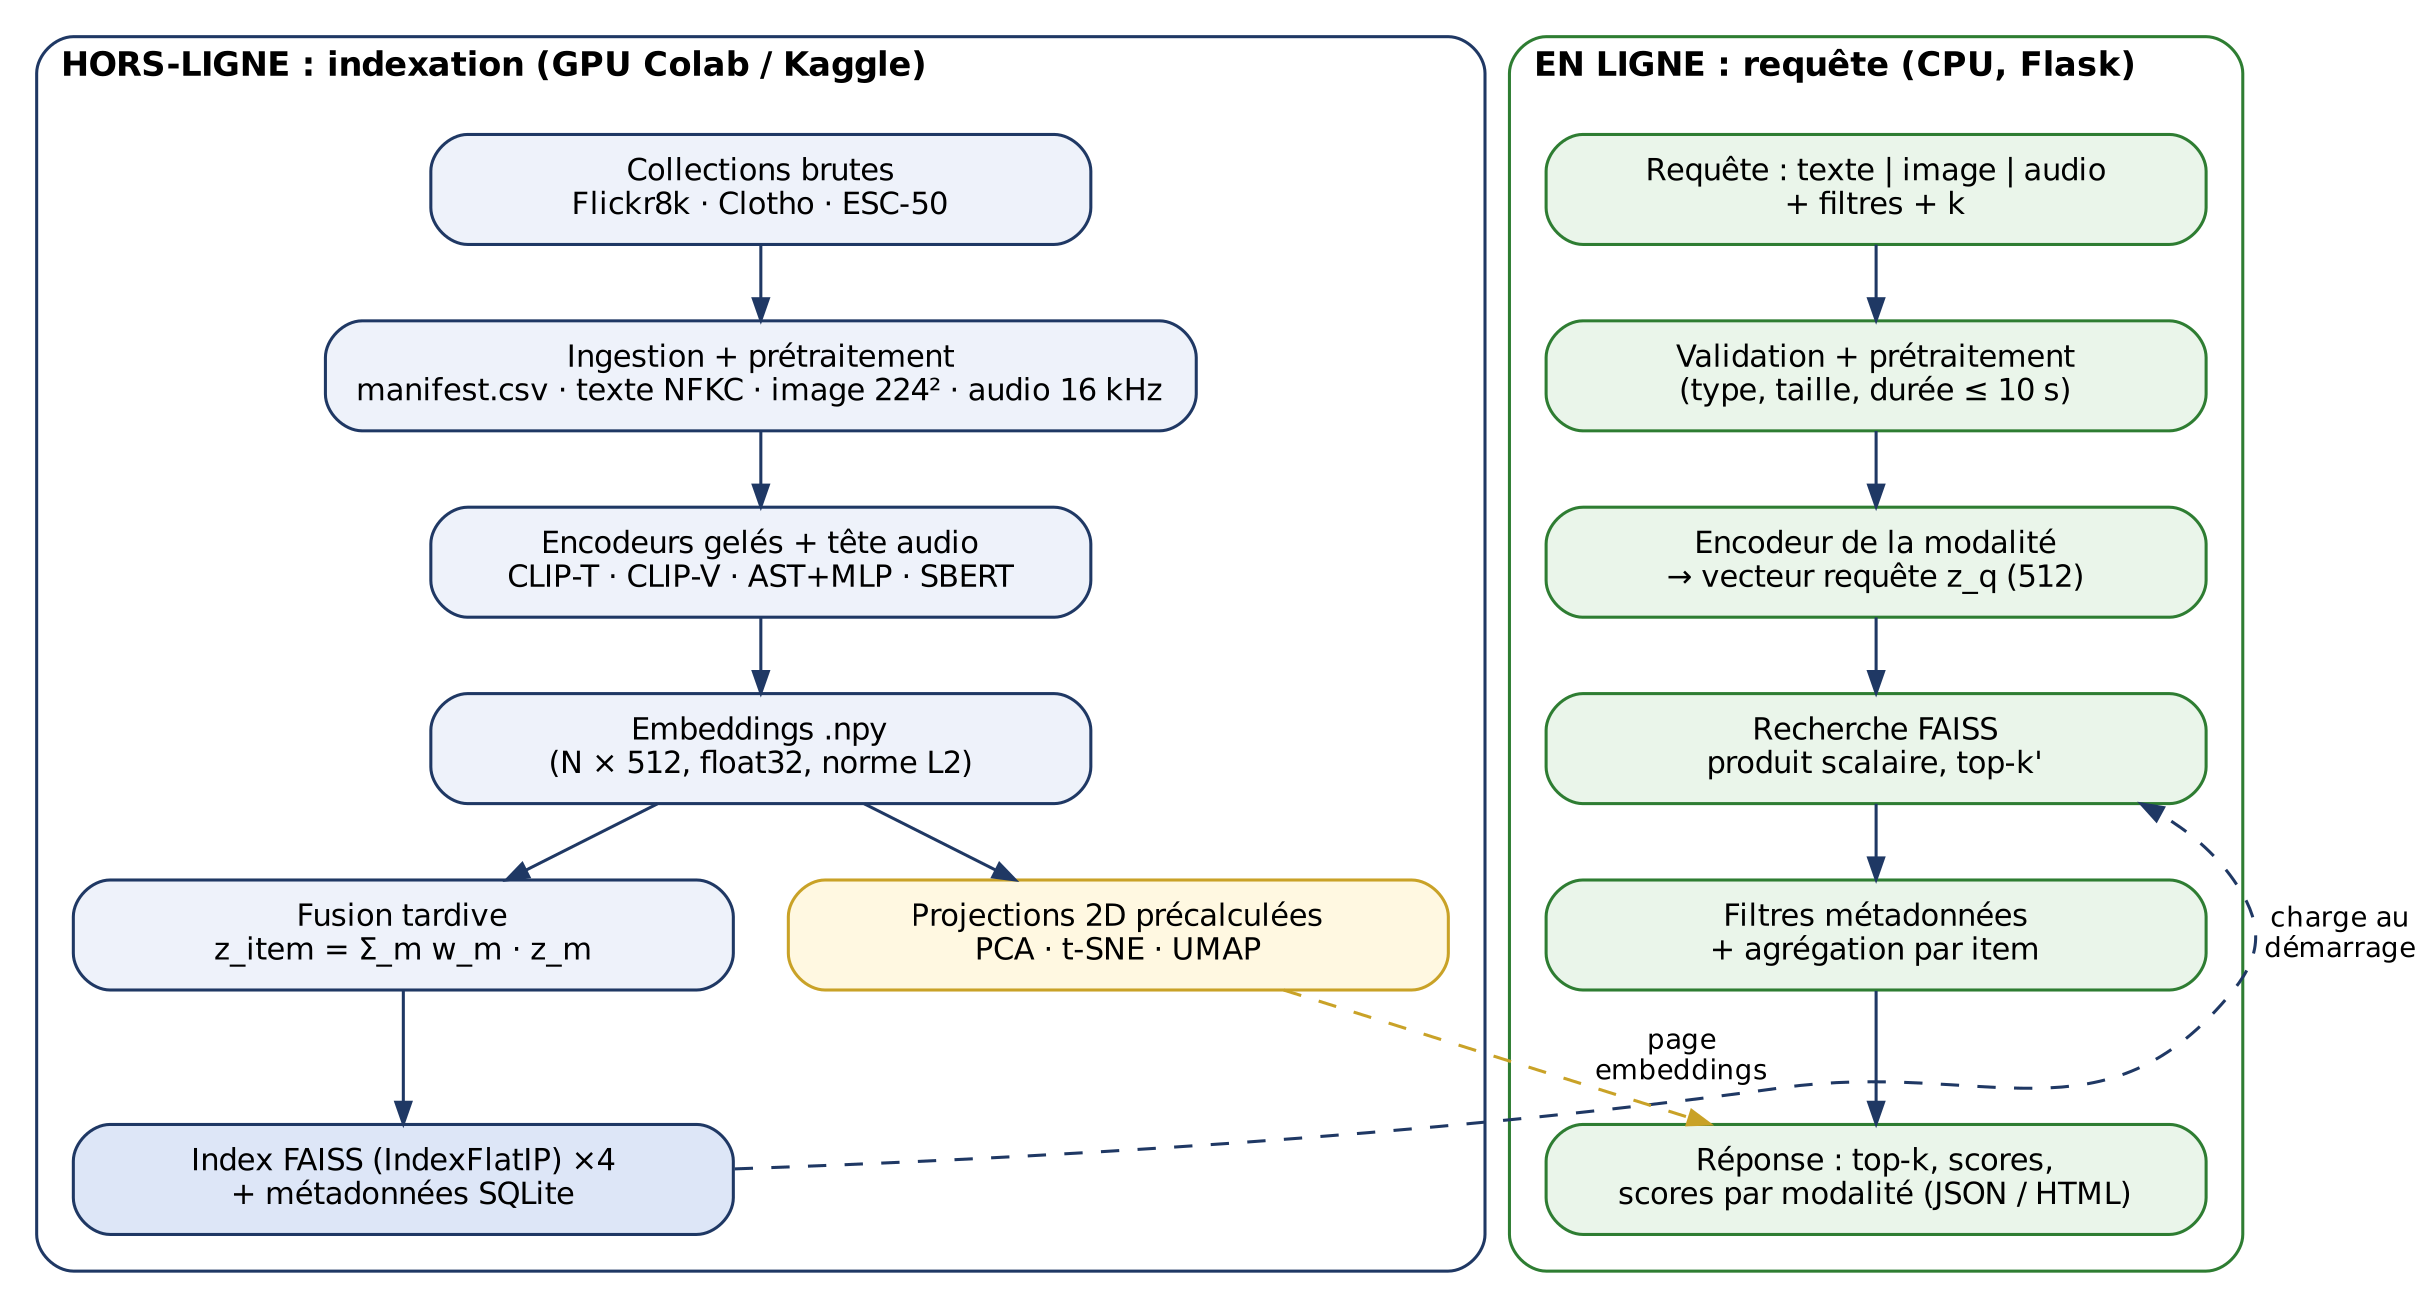
\includegraphics[width=\linewidth]{architecture.png}
\caption{Chaîne complète : de la collection brute à la réponse Flask.}
\end{figure}

\subsection{Index et recherche}
Quatre index FAISS exacts (\texttt{IndexFlatIP}) : images (8\,091), audio ($\approx$ 6\,000), légendes
($\approx$ 70\,455) et items fusionnés ($\approx$ 14\,091), soit $\approx 202$\,Mo. Routage : texte$\to$items fusionnés ;
image$\to$légendes agrégées par item ; audio$\to$items fusionnés (audio$\to$contenu) ; le mode mono-modal interroge les index
séparés. Les filtres (modalité, dataset, split, label, score minimal) sont appliqués par pré-filtrage exact.

\subsection{Budget de calcul}
\begin{table}[ht]\centering\small
\begin{tabular}{@{}lccc@{}}
\toprule
Encodeur & MACs & FLOPs & Temps CPU estimé\\
\midrule
CLIP texte ($d=512$, $T=77$) & $2{,}98\cdot10^9$ & $5{,}96\cdot10^9$ & $\approx0{,}12$ s\\
CLIP image ($d=768$, $T=50$) & $4{,}29\cdot10^9$ & $8{,}59\cdot10^9$ & $\approx0{,}17$ s\\
AST, 10 s ($d=768$, $T=1212$) & $1{,}30\cdot10^{11}$ & $2{,}60\cdot10^{11}$ & $\approx5{,}2$ s\\
\bottomrule
\end{tabular}
\caption{Coût par requête (hypothèse : 50 GFLOPS effectifs ; \TODO{mesurer sur la machine de démonstration}).}
\end{table}

\subsection{Application Flask}
Routes : \texttt{POST /api/search}, \texttt{GET /api/item/<id>}, \texttt{GET /media/<id>}, \texttt{GET /api/embeddings},
\texttt{POST /api/classify}, \texttt{GET /api/health}. Fonctions : indexation d'une collection, barre de recherche, upload
image ou audio, top-$k$, scores de similarité (cosinus) et scores par modalité, filtres, page de visualisation des embeddings
(PCA, t-SNE \cite{vandermaaten2008tsne}, UMAP \cite{mcinnes2018umap}).
\TODO{3 captures d'écran : recherche texte, upload image, page embeddings coloriée par classe ESC-50.}

\section{Expériences et résultats}\label{sec:resultats}
\subsection{Protocole}
Texte$\to$image sur le test de Flickr8k ($1\,000$ images, $5\,000$ requêtes), leave-one-out, $w$ réglé sur la validation.
Les systèmes comparés : mono-texte (SBERT et CLIP), mono-image (CLIP), fusion tardive, fusion précoce.
\TODO{n et K exacts, poids $w$ retenu, matériel.}

\subsection{Mono-modal contre multimodal}
\inputopt{../artifacts/figures/results_tables.tex}
\figopt{fig_mono_vs_multi.png}{0.75}{Texte $\to$ image : mono-modal contre multimodal.}
\TODO{commenter : le multimodal apporte-t-il un gain, de quelle taille, avec quel intervalle de confiance ? comparer au hasard.}

\subsection{Réglage de la fusion et ablations}
\figopt{fig_fusion_weights.png}{0.6}{Réglage de $w$ sur la validation (image et audio).}
\figopt{fig_dim_ablation.png}{0.6}{Ablation de la dimension $d$.}
\TODO{commenter le $w$ retenu, l'effet de $d$, la fusion précoce par rapport à la tardive.}

\subsection{\texorpdfstring{Image$\leftrightarrow$texte, audio$\leftrightarrow$texte, audio$\to$image}{Image-texte, audio-texte, audio vers image}}
\TODO{tableaux R@K, P@K, MRR depuis \texttt{results.json} ; audio$\to$image : donner la précision@10, le taux de base et le
gain par classe (proxy, voir limites).}

\subsection{Visualisation de l'espace commun}
\figopt{fig_proj_pca.png}{0.48}{PCA.}\hfill\figopt{fig_proj_tsne.png}{0.48}{t-SNE.}
\figopt{fig_proj_umap.png}{0.48}{UMAP.}
\TODO{commenter l'alignement des modalités et le « modality gap » \cite{liang2022gap} observé.}

\subsection{Étude de cas}
\TODO{choisir 2 succès et 2 échecs dans \texttt{case\_studies.json}, montrer requête, image attendue, top-5, expliquer l'échec.}

\section{Discussion, biais et limites}\label{sec:discussion}
\subsection{Biais et limites de la fusion}
\begin{table}[ht]\centering\small
\begin{tabular}{@{}p{3.2cm}p{5.6cm}p{5.6cm}@{}}
\toprule
Source & Constat à documenter & Mesure ou atténuation\\
\midrule
Biais des jeux de données & légendes en anglais, culture occidentale, scènes de personnes et d'animaux surreprésentées & \texttt{bias\_report.json} : part par groupe, Recall par groupe ($n\ge30$, IC 95\,\%)\\
Déséquilibre des modalités & texte pivot ; image et audio jamais appariés ; 8\,091 images contre $\approx$ 6\,000 clips & comparaison audio seul / fusion ; perspective : paires image--audio\\
Dérive de domaine & Clotho (clips de 15 à 30 s) contre ESC-50 (5 s, sons isolés) ; pré-entraînement AudioSet & zero-shot ESC-50 ; recouvrement Freesound à signaler\\
Alignement imparfait & écart entre modalités \cite{liang2022gap}, concentration des voisins (\emph{hubness}) \cite{radovanovic2010hubs} & PCA/UMAP colorées par modalité ; scores non calibrés entre modalités\\
Fusion tardive & poids global $w$ non adaptatif ; moyenne de légendes qui dilue les détails & ablation de $w$ ; fusion précoce ; re-ranking par attention croisée\\
Évaluation & leave-one-out simule des légendes absentes de la requête réelle ; proxy audio$\to$image sans vérité terrain ; une seule graine & intervalles de confiance ; plusieurs graines ; évaluation humaine\\
\bottomrule
\end{tabular}
\caption{Biais et limites, avec la mesure correspondante.}
\end{table}
\figopt{fig_bias_groups.png}{0.7}{Texte $\to$ image par groupe thématique : fusion contre image seule.}
\TODO{3 paragraphes : (1) biais de données chiffrés, (2) écarts de Recall entre groupes (groupes avec $n\ge30$), (3) ce que la
fusion corrige ou aggrave.}

\subsection{Perspectives}
Fine-tuning partiel d'AST, baseline LAION-CLAP \cite{wu2023clap}, légendes multilingues (français), calibration des scores entre
modalités, annotation humaine image--audio, index approché si la collection dépasse $10^6$ éléments.

\section{Conclusion}
\TODO{Bilan en 5 phrases : (1) ce qui a été construit ; (2) résultat principal chiffré (mono-modal contre multimodal) ;
(3) résultat audio et zero-shot ; (4) limite principale ; (5) ouverture. Aucune affirmation sans chiffre de \texttt{results.json}.}


\bibliographystyle{plain}
\bibliography{refs}

\appendix
\section{Notations}
\begin{tabular}{@{}ll@{}}
\toprule
Symbole & Signification\\
\midrule
$d=512$ & dimension de l'espace commun\\
$z\in\R^d,\ \norm{z}=1$ & embedding normalisé (image, texte ou audio)\\
$\tau$ & température de la perte contrastive, $\tau=e^{-\text{logit\_scale}}$\\
$w_m$ & poids de la modalité $m$ dans la fusion tardive, $\sum_m w_m=1$\\
$\bar z_i$ & vecteur fusionné de l'item $i$\\
$K=5$ & nombre de légendes par item\\
R@K, P@K & Recall et Precision au rang $K$\\
\bottomrule
\end{tabular}

\section{Reproductibilité}
Dépôt Git (tag \texttt{rendu}), \texttt{requirements.txt} épinglé, graine 42, procédure : \texttt{README.md}.
\begin{verbatim}
make install && make data && make embed && make train && make fusion
make index && make projections && make eval && make figures && make app
\end{verbatim}
\TODO{versions exactes (python, torch, transformers, faiss), matériel utilisé, durée de chaque étape.}

\end{document}
